\documentclass[paper=a4,oneside,fontsize=12pt,DIV=14,headings=normal,parskip=half,headsepline,numbers=noendperiod]{scrreprt}
\usepackage[T1]{fontenc}
\usepackage[utf8]{inputenc}
\usepackage[english]{babel}
\usepackage{lmodern}
\usepackage[bitstream-charter]{mathdesign}
\usepackage[scaled=0.92]{helvet}
\usepackage{microtype}
\usepackage[onehalfspacing]{setspace}
\usepackage[outer=25mm,inner=30mm,top=26mm,bottom=28mm,heightrounded=true]{geometry}
\usepackage{mathtools,bm,amsthm}
\usepackage{booktabs,tabularx,array}
\usepackage{graphicx,float}
\usepackage[automark]{scrlayer-scrpage}
\usepackage[hidelinks]{hyperref}
\usepackage[nameinlink,noabbrev]{cleveref}
\addtokomafont{disposition}{\normalfont\bfseries}
\setkomafont{pageheadfoot}{\normalfont\small}
\ihead{Hybrid SDA Core Argument}\ohead{\pagemark}\cfoot{}
\setlength{\emergencystretch}{2em}
\renewcommand{\arraystretch}{1.18}
\newcommand{\vct}[1]{\bm{#1}}
\newcommand{\mat}[1]{\bm{#1}}
\newcommand{\T}{\mathsf{T}}
\newtheorem{proposition}{Proposition}[chapter]

\begin{document}
\begin{titlepage}
\centering\vspace*{3cm}
{\sffamily\bfseries\fontsize{23}{28}\selectfont
Hybrid Sphere Decoding with Embedded Initialization and Explicit Pruning\par}
\vspace{0.6cm}
{\sffamily\fontsize{16}{20}\selectfont
Core Mathematical Argument and Controlled Experimental Evidence\par}
\vfill
\begin{minipage}{0.84\textwidth}\small
This concise report retains only the evidence required to justify the proposed
hybrid SDA: complete-sequence equivalence, embedded upper-bound quality,
explicit optimality-certification efficiency, and total hybrid search effort.
Exploratory diagnostics are maintained separately in the detailed analysis
report and are intentionally omitted here.
\end{minipage}
\vfill{\large October 2026\par}
\end{titlepage}
\pagenumbering{roman}\tableofcontents\clearpage\pagenumbering{arabic}

\chapter{Research Question and Claim}

The controller optimizes a binary switching sequence
\begin{equation}
 \vct U=[S_{a,1},S_{b,1},S_{c,1},\ldots,S_{a,N_p},S_{b,N_p},S_{c,N_p}]^\T,
 \qquad \vct U\in\{0,1\}^{3N_p},
\end{equation}
with $N_p=5$.  Two representations of the zero-vector objective are available.
The \emph{explicit} formulation adds $\lambda_z$ when a completed three-phase
switching vector is $000$ or $111$.  The \emph{embedded} formulation absorbs
an equivalent quadratic expression into the matrix factor used by the sphere
decoder.

The proposed method does not select one representation for the entire solver.
It uses their complementary properties:
\begin{equation}
 \boxed{\text{embedded Babai initialization}
 +\text{ explicit branch-and-bound search}.}
\end{equation}
The academic argument consists of three claims:
\begin{enumerate}
 \item complete-sequence equivalence permits a candidate to be transferred
 safely between the formulations;
 \item the embedded representation provides a better initial feasible upper
 bound;
 \item the explicit representation certifies optimality with fewer nodes once
 initializer quality is controlled.
\end{enumerate}

\paragraph{Terminology.}
An \emph{incumbent} is the best complete feasible sequence found so far; its
cost is the current upper bound or sphere radius $R$.  A \emph{prefix} is an
incomplete sequence containing the first $i$ binary decisions.  Its partial
metric $P_i$ is a lower bound used for pruning.  A node is pruned when
$P_i>R$.  Thus upper-bound quality and prefix-bound quality are distinct
properties.

\chapter{Claim 1: Complete-Sequence Equivalence}

For one three-phase vector define
\begin{equation}
 m=S_a+S_b+S_c,\qquad m\in\{0,1,2,3\}.
\end{equation}
The explicit zero-vector cost is represented exactly on the binary domain by
\begin{equation}
 J_{\mathrm{z,exp}}(m)=\frac{\lambda_z}{2}(m-1)(m-2).
\end{equation}
The embedded centered quadratic is
\begin{equation}
 J_{\mathrm{z,emb}}(m)=\frac{\lambda_z}{2}(m-1.5)^2.
\end{equation}
Expanding both expressions gives
\begin{equation}
 J_{\mathrm{z,emb}}(m)
 =J_{\mathrm{z,exp}}(m)+\frac{\lambda_z}{8}.
\end{equation}

\begin{proposition}[Leaf-level equivalence]
For every complete binary sequence,
\begin{equation}
 J_{\mathrm{emb}}(\vct U)
 =J_{\mathrm{exp}}(\vct U)+C,
 \qquad C=\frac{N_p\lambda_z}{8}.
 \label{eq:leaf_equivalence}
\end{equation}
Consequently, both formulations have the same minimizer set.
\end{proposition}
\begin{proof}
The per-block difference is independent of $m$.  Summation over $N_p$ blocks
adds the same constant to every feasible complete sequence and therefore
preserves every objective ordering.
\end{proof}

For $N_p=5$ and $\lambda_z=10{,}000$,
\begin{equation}
 C=6250.
\end{equation}
The numerical evidence is deliberately minimal but exhaustive at the selected
analysis points: all $2^{15}$ complete sequences exhibited the same difference
$6249.99992$ to floating-point accuracy.  All paired closed-loop samples also
returned identical optimal switching sequences.  This establishes that an
embedded Babai sequence is a valid candidate for the explicit problem once its
cost is reevaluated under the explicit objective.

\chapter{Claim 2: Embedded Initialization Provides a Better Upper Bound}

Let the initial optimality gap be
\begin{equation}
 G_0=R_0-J^\star\geq0,
 \label{eq:initial_gap}
\end{equation}
where $R_0$ is the feasible initial incumbent obtained by evaluating the
initializer's switching sequence under the objective being searched, and
$J^\star$ is the globally optimal cost in the corresponding representation.
A smaller $G_0$ means a better initial feasible upper bound; $G_0=0$ means
that the initializer already supplies an optimal sequence.

The native explicit implementation selects Round, Shift, or Babai using only
the quadratic tracking distance and adds the explicit zero-vector/dead-time
cost afterward.  Consequently, a sequence that is geometrically close to the
unconstrained center can still receive a large discrete penalty.  The embedded
Babai construction already includes the zero-vector term in its geometry.

\begin{table}[H]
\centering
\caption{Initial upper-bound quality over 500 transactions per torque.}
\label{tab:upper_bound}
\begin{tabular}{lrrrr}
\toprule
&\multicolumn{2}{c}{Native explicit}&\multicolumn{2}{c}{Embedded Babai}\\
Torque & Median $G_0$ & Optimal at start & Median $G_0$ & Optimal at start\\
\midrule
10~Nm & 49279 & 0\% & $\approx0$ & 51.8\%\\
50~Nm & 39947 & 0\% & 2.55 & 49.2\%\\
90~Nm & 39879 & 0\% & 57.12 & 40.0\%\\
\bottomrule
\end{tabular}
\end{table}

\begin{figure}[H]
\centering
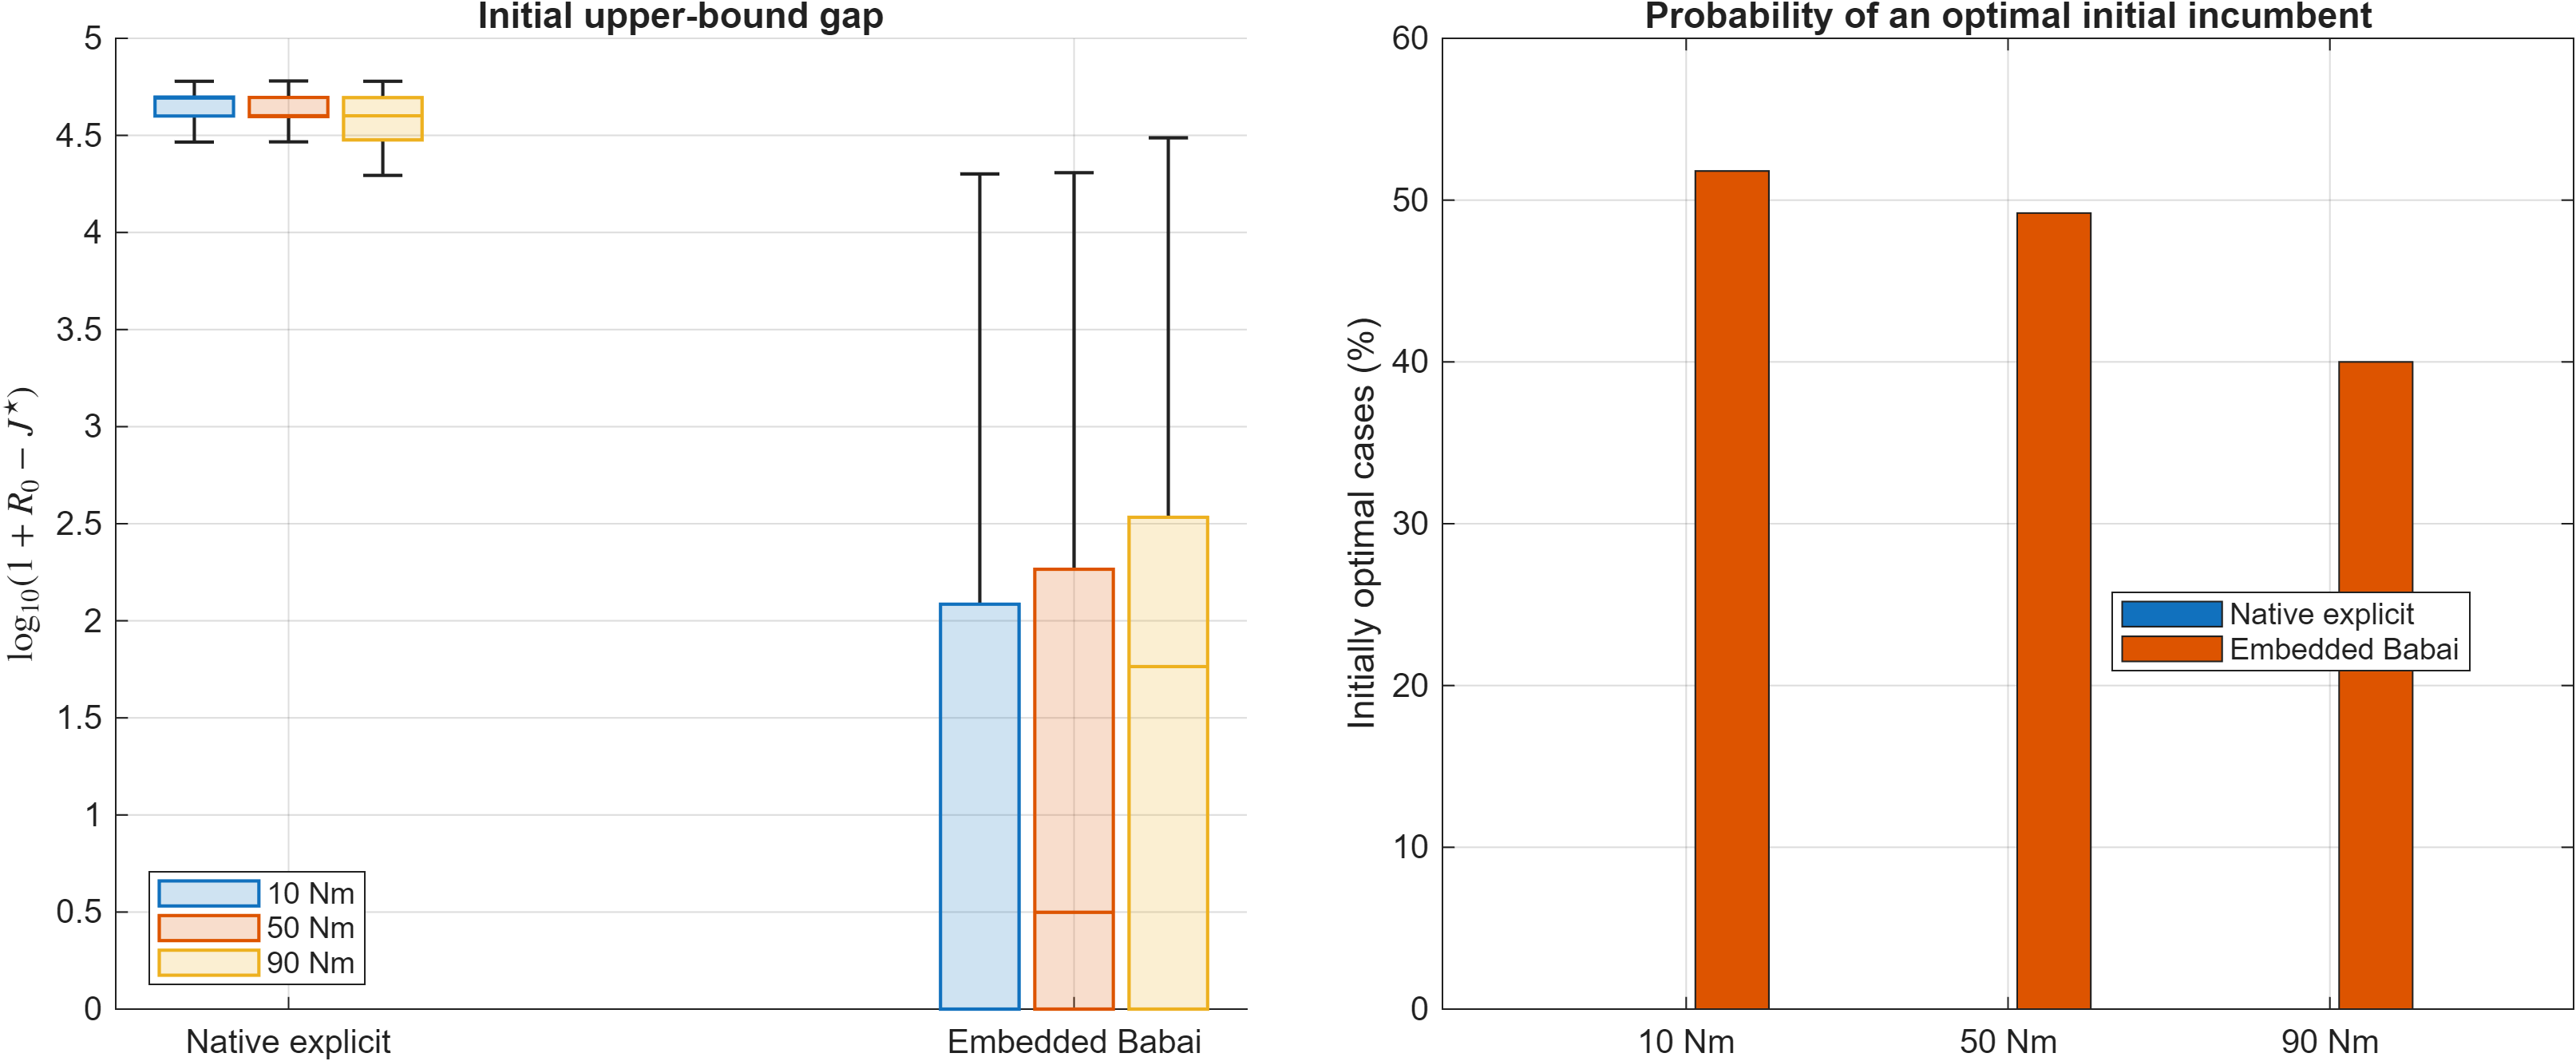
\includegraphics[width=\textwidth]{../hybrid_results/core_upper_bound_evidence.png}
\caption{Direct evidence for the embedded upper-bound claim.  Left: initial
optimality gap from \cref{eq:initial_gap}, displayed as
$\log_{10}(1+G_0)$.  Right: percentage of transactions in which the initial
candidate is already globally optimal.}
\label{fig:upper_bound}
\end{figure}

The result supports a scoped empirical statement: under the investigated
horizon, weight, variable ordering, and operating conditions, the embedded
Babai construction gives a substantially tighter initial upper bound.  It does
not claim that embedded Babai is optimal for every possible state.

\chapter{Claim 3: Explicit Search Certifies Optimality More Efficiently}

At depth $i=3q$, exactly $q$ complete three-phase switching vectors are known.
For the implemented forward ordering, the same-prefix metrics satisfy
\begin{equation}
 P_{3q}^{\mathrm{emb}}-P_{3q}^{\mathrm{exp}}
 =q\frac{\lambda_z}{8}.
\end{equation}
After normalizing the complete embedded objective by
$C=N_p\lambda_z/8$,
\begin{equation}
 P_{3q}^{\mathrm{exp}}-\widetilde P_{3q}^{\mathrm{emb}}
 =(N_p-q)\frac{\lambda_z}{8}>0,
 \qquad q<N_p.
 \label{eq:prefix_advantage}
\end{equation}
Thus the explicit metric is tighter at the completed switching-vector
boundaries.  Numerically, the accumulated offsets at depths
$3,6,9,12,15$ are exactly $1250,2500,3750,5000,6250$ for all enumerated
prefixes.

The strongest experimental isolation is the oracle comparison.  Both searches
are initialized with the already known optimal sequence.  Initialization
quality is therefore identical and cannot explain the remaining node-count
difference.

\begin{table}[H]
\centering
\caption{Mean nodes required when the globally optimal incumbent is supplied
before search.}
\label{tab:oracle}
\begin{tabular}{lrrr}
\toprule
Method & 10~Nm & 50~Nm & 90~Nm\\
\midrule
Oracle explicit & 160.49 & 161.12 & 150.97\\
Oracle embedded & 1123.00 & 1137.90 & 1010.40\\
Explicit reduction & 85.7\% & 85.8\% & 85.1\%\\
\bottomrule
\end{tabular}
\end{table}

The explicit search therefore requires only approximately 14--15\% of the
embedded node count to certify the same already known optimum.  Combined with
\cref{eq:prefix_advantage}, this provides direct mathematical and controlled
experimental evidence for the explicit proof-stage advantage.  The statement
is scoped to the implemented factorization and variable ordering; universal
node dominance at every intermediate depth is not claimed.

\section{Secondary analysis of the Cholesky-factor distribution}
The recursive increment can be written in terms of the conditional center
\begin{equation}
 c_i=\frac{(H U_{\mathrm{unc}})_i-H_{i,1:i-1}U_{1:i-1}}{H_{ii}}
\end{equation}
as
\begin{equation}
 \Delta P_i=H_{ii}^2(U_i-c_i)^2.
 \label{eq:level_increment}
\end{equation}
Thus, the row norm alone is not the level-wise discrimination gain.  The
diagonal magnitude $|H_{ii}|$ scales the present binary decision, while the
preceding row coefficients determine how strongly the center depends on the
already selected prefix.  To separate these effects, define
\begin{equation}
 \kappa_i=\frac{\|H_{i,1:i-1}\|_2}{|H_{ii}|}.
\end{equation}

The row norm, diagonal magnitude, and coupling ratio were evaluated on the same
1500 transactions used by the oracle experiment.  Their formulation
differences were correlated with
\begin{equation}
 \Delta N_{\mathrm{oracle}}
 =N_{\mathrm{oracle,emb}}-N_{\mathrm{oracle,exp}}
\end{equation}
using Spearman rank correlation.

\begin{figure}[H]
\centering
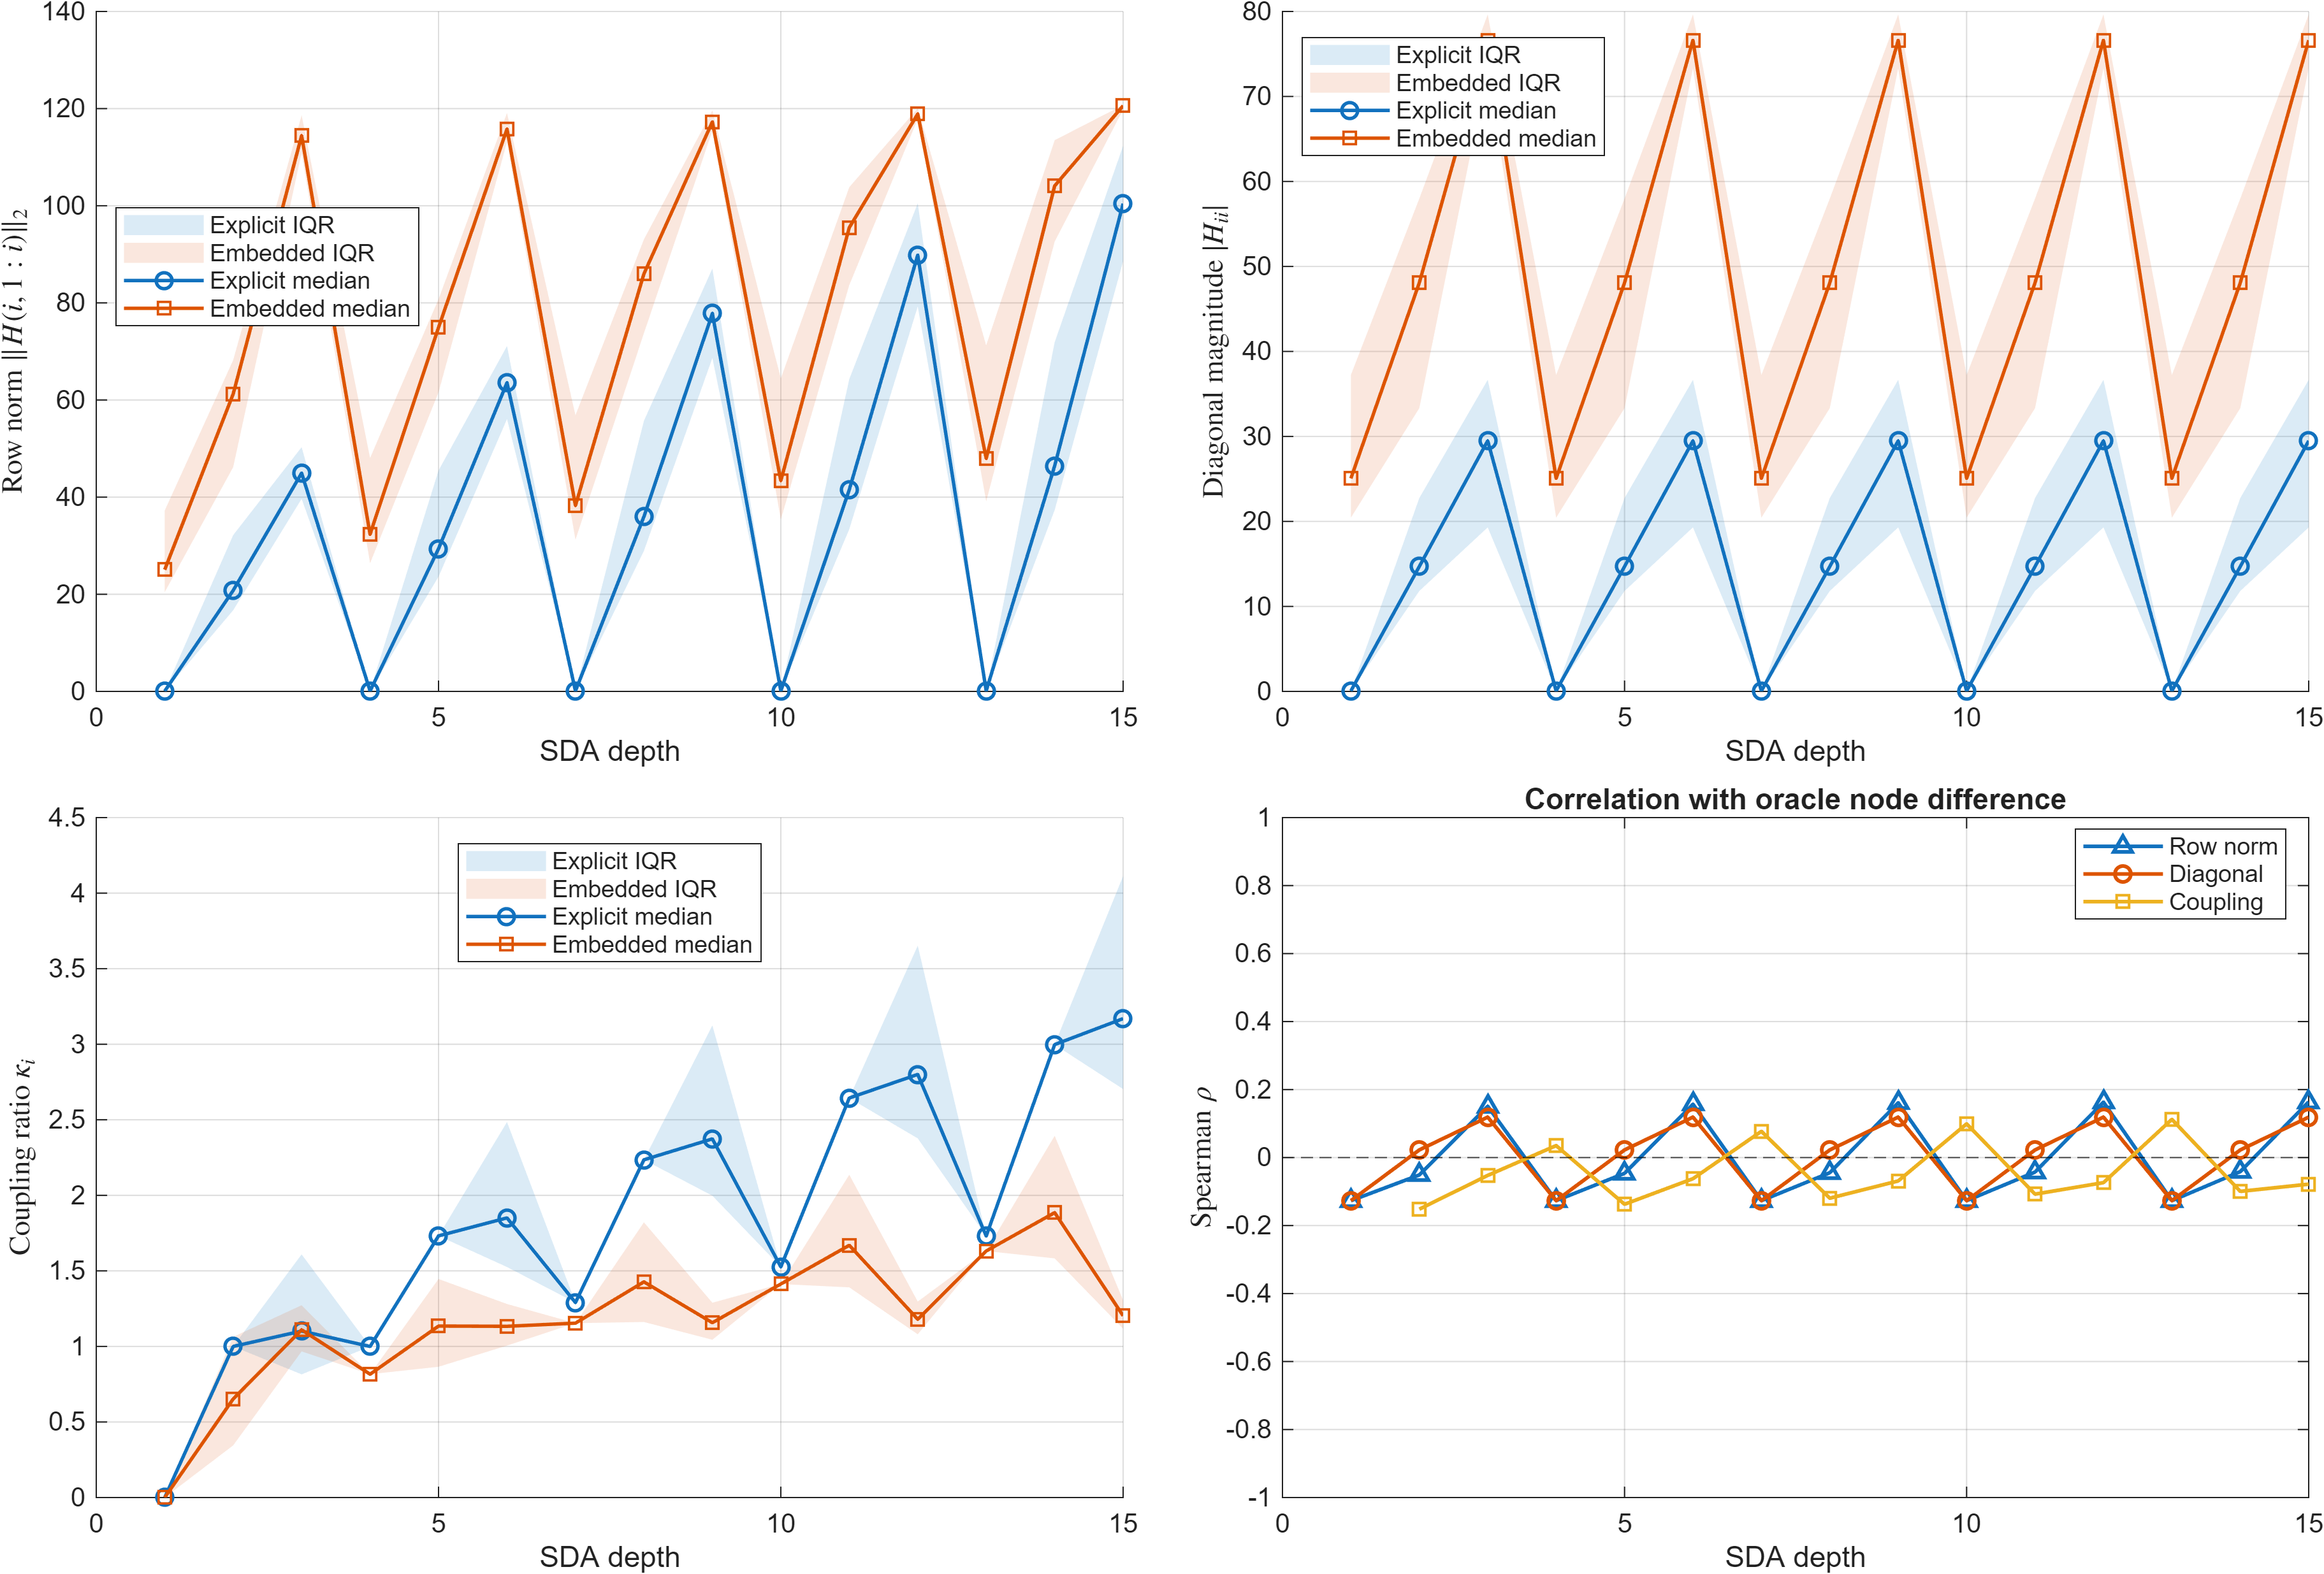
\includegraphics[width=\textwidth]{../hybrid_results/H_factor_distribution_and_correlation.png}
\caption{Cholesky-factor structure under a common optimal incumbent.  Shaded
regions are interquartile ranges over all sampled transactions.  The lower
right panel correlates the embedded--explicit difference of each structural
quantity with the paired oracle node-count difference.}
\label{fig:H_structure}
\end{figure}

\begin{table}[H]
\centering
\caption{Largest absolute depth-wise Spearman correlation with the oracle node
difference.  Small $p$-values reflect the sample count and do not imply a large
effect size.}
\label{tab:H_correlation}
\begin{tabular}{lrrr}
\toprule
Structural quantity & Maximum $|\rho|$ & Depth & Interpretation\\
\midrule
Row norm difference & 0.164 & 15 & weak association\\
Diagonal difference & 0.127 & repeated block positions & weak association\\
Coupling-ratio difference & 0.152 & 2 & weak association\\
\bottomrule
\end{tabular}
\end{table}

The embedded factor clearly redistributes level-wise scaling: it has larger row
norms and diagonal magnitudes, while the explicit factor develops larger
normalized coupling at many deeper levels.  Nevertheless, all observed
correlations satisfy $|\rho|<0.17$.  These simple marginal descriptors therefore
do not explain the order-of-magnitude oracle node difference on their own.
Their influence acts jointly through the path-dependent centers in
\cref{eq:level_increment}, enumeration order, and accumulated prefix bounds.
This result rules out the overly simple explanation that the embedded search is
slower merely because its rows are ``flatter'' or larger.  The primary evidence
remains the block-boundary prefix relation and the controlled oracle experiment.

\chapter{Hybrid Algorithm and Correctness}

The hybrid first computes
\begin{equation}
 \vct U_{\mathrm B}^{\mathrm{emb}}
 =\operatorname{Babai}(\mat H_{\mathrm{emb}},
                       \vct U_{\mathrm{unc,emb}}).
\end{equation}
It then reevaluates this sequence under the explicit objective:
\begin{equation}
 R_{0,\mathrm{hyb}}
 =J_{\mathrm{exp}}(\vct U_{\mathrm B}^{\mathrm{emb}}),
\end{equation}
and starts the original explicit SDA using this sequence and radius.

\begin{proposition}[Global optimality preservation]
If the explicit SDA terminates without reaching its node limit, replacing its
native initial candidate by the embedded Babai candidate does not change the
globally optimal output.
\end{proposition}
\begin{proof}
$\vct U_{\mathrm B}^{\mathrm{emb}}$ is a complete feasible binary sequence, so
its explicit cost is an upper bound on the explicit optimum.  The subsequent
explicit branch-and-bound algorithm and all of its valid lower bounds are
unchanged.  The initializer can change the search order and pruning amount but
cannot remove a branch capable of improving the incumbent.
\end{proof}

\chapter{Controlled Ablation Result}

\section{Dataset, pairing, and sample selection}
All results in this chapter originate from the same SDI archive,
\texttt{embedded\_H.mldatx}.  The archive contains 40,000 SDA transactions for
each of the following six closed-loop runs:
\begin{equation}
\begin{aligned}
 &\texttt{original\_10NM},\quad
  \texttt{original\_50NM},\quad
  \texttt{original\_90NM},\\
 &\texttt{embedded\_H\_10NM},\quad
  \texttt{embedded\_H\_50NM},\quad
  \texttt{embedded\_H\_90NM}.
\end{aligned}
\end{equation}
The auxiliary run \texttt{original\_no\_zero\_lambda\_10NM} is not used in the
hybrid or oracle comparison.

The interval before $t=0.05$~s is excluded to avoid the initial startup
transient.  From the remaining transactions, 500 indices are selected at
uniformly spaced positions for each torque condition.  The same indices are
used for the original and embedded runs, producing
\begin{equation}
 3\ \text{torque conditions}\times500
 =1500
\end{equation}
paired physical operating points.  ``Paired'' means that the two formulations
are compared at the same torque label, controller time, and transaction index.
The selection is deterministic and is not based on the resulting node count.

For every selected transaction, the replay input contains the logged factor
$H$, unconstrained center $U_{\mathrm{unc}}$, previous switching sequence,
compensated current, current-increment matrices, node limit, zero-vector and
dead-time weights, dead-time ratio, and current-sign margin.  Each formulation
retains its own logged $H$ and $U_{\mathrm{unc}}$; only the physical transaction
index is paired.

\section{Meaning of the five configurations}
\Cref{tab:configurations} states exactly which data and initializer are used by
each configuration.

\begin{table}[H]
\centering
\caption{Inputs and initialization used in the ablation study.}
\label{tab:configurations}
\begin{tabularx}{\textwidth}{lXXX}
\toprule
Configuration & Matrix and center & Initial complete sequence & Purpose\\
\midrule
Native explicit
& From the paired \texttt{original} run
& Best quadratic Round/Shift/Babai candidate selected by the production logic
& Production reference\\

Native embedded
& From the paired \texttt{embedded\_H} run
& Best quadratic Round/Shift/Babai candidate in embedded geometry
& Embedded reference\\

Hybrid
& Explicit $H$ and center for search; embedded $H$ and center only for Babai
& Embedded Babai sequence, reevaluated under the explicit objective
& Proposed implementable method\\

Oracle explicit
& From the paired \texttt{original} run
& Logged globally optimal sequence $U^\star$
& Isolate explicit certification effort\\

Oracle embedded
& From the paired \texttt{embedded\_H} run
& The same logged globally optimal binary sequence $U^\star$
& Isolate embedded certification effort\\
\bottomrule
\end{tabularx}
\end{table}

The oracle configurations do not constitute a separate dataset.  They replay
the same 1500 paired transactions but replace the practical initializer by the
already known logged optimum.  Each oracle recomputes the cost of $U^\star$
under its own objective:
\begin{equation}
 R_{0,\mathrm{oracle,exp}}=J_{\mathrm{exp}}(U^\star),
 \qquad
 R_{0,\mathrm{oracle,emb}}=J_{\mathrm{emb}}(U^\star).
\end{equation}
The numerical radii therefore differ by 6250; the shared quantity is the
optimal binary sequence, not the raw radius.  Oracle results are used only to
remove initializer quality as a confounding variable.  Because they use the
known solution, they are diagnostic lower baselines and are not presented as
deployable controllers.

\section{Replay validation}
Every replayed configuration is accepted only if its final cost and switching
sequence agree with the logged reference within numerical tolerance.  Thus the
reported node counts compare alternative search procedures on the same solved
optimization instances rather than different control trajectories.  The
closed-loop plant is not resimulated during this offline analysis.

Five configurations were evaluated on the same 500 transactions per torque:
native explicit, native embedded, the implementable hybrid, and two diagnostic
oracle searches.  Every configuration reproduced the logged optimal sequence
and cost.

\begin{table}[H]
\centering
\caption{Total search effort.  Entries are mean nodes with Q95 in parentheses.}
\label{tab:ablation}
\begin{tabular}{lrrr}
\toprule
Method & 10~Nm & 50~Nm & 90~Nm\\
\midrule
Native explicit & 451.96 (919) & 466.67 (1033) & 442.48 (867)\\
Native embedded & 1140.90 (1794) & 1179.00 (1845) & 1100.20 (1745)\\
Hybrid & \textbf{182.66 (489)} & \textbf{191.49 (500)} & \textbf{199.92 (504)}\\
Oracle explicit & 160.49 (427) & 161.12 (380) & 150.97 (313)\\
Oracle embedded & 1123.00 (1746) & 1137.90 (1808) & 1010.40 (1662)\\
\bottomrule
\end{tabular}
\end{table}

\begin{figure}[H]
\centering
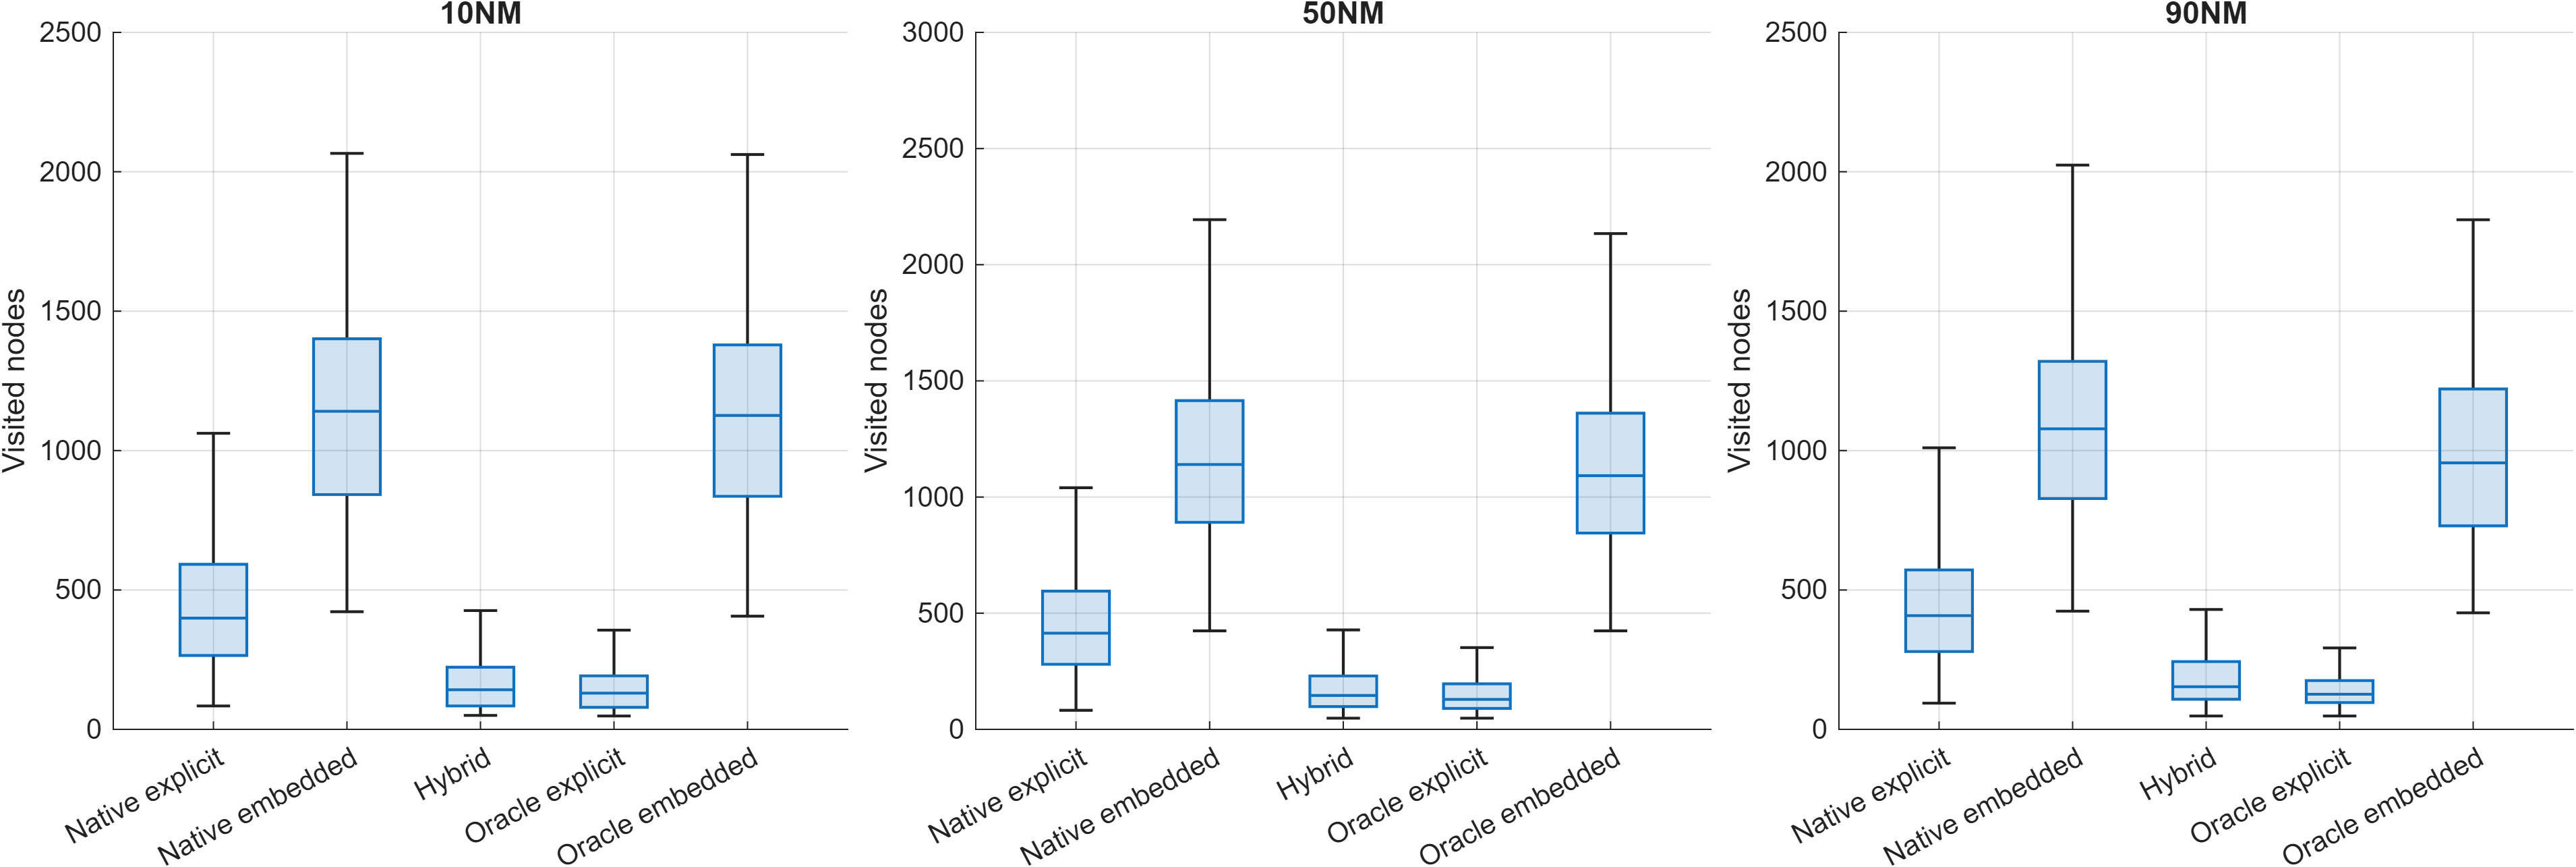
\includegraphics[width=\textwidth]{../hybrid_results/core_node_count_ablation.png}
\caption{Node-count distributions for the complete ablation.  The hybrid is
the lowest-node implementable configuration and approaches the diagnostic
oracle-explicit baseline.}
\label{fig:node_ablation}
\end{figure}

Relative to the native explicit solver, the hybrid reduces mean nodes by
59.6\%, 59.0\%, and 54.8\% at 10, 50, and 90~Nm.  Relative to native embedded,
the reductions are 84.0\%, 83.8\%, and 81.8\%.  These reductions are obtained
without changing the returned globally optimal switching sequence.

\chapter{Closed-Loop Deployment Validation}

The offline replay isolates the search mechanism, but it does not by itself
show that the complete Simulink feedback loop preserves the same behavior.
The hybrid solver was therefore deployed in
\texttt{FCSMPC\_double\_vector\_2025b}.  Its 10-kHz stage forms both factors,
its 40-kHz stage forms both matched unconstrained centers after one current
reconstruction, and its SDA stage uses the embedded pair only for Babai before
returning to the explicit pair for search.  The original and embedded-only
paths were commented out during the hybrid runs.

The archive \texttt{hybrid\_SDA.mldatx} contains one-second runs at 10, 50,
and 90~Nm.  After excluding $t<0.05$~s, each condition contributes 38,001
transactions.  These transactions were paired by timestamp with the original
and embedded runs in \texttt{embedded\_H.mldatx}, giving 114,003 comparisons.
All methods returned \texttt{optimal=true}, and none reached the 10,000-node
limit.

\section{Time-domain overview}

Figures~\ref{fig:time_nodes_10}--\ref{fig:time_nodes_90} provide a direct view
of the three node-count signals before they are reduced to statistical
summaries.  Since plotting every 40-kHz optimizer call would form an opaque
band, the one-second record is divided into non-overlapping 1-ms bins.  Each
displayed point is the arithmetic mean of the approximately 40 synchronized
transactions in that bin.  This operation is for visualization only; the
tables and distributional results retain every transaction after 50~ms.

\begin{figure}[H]
\centering
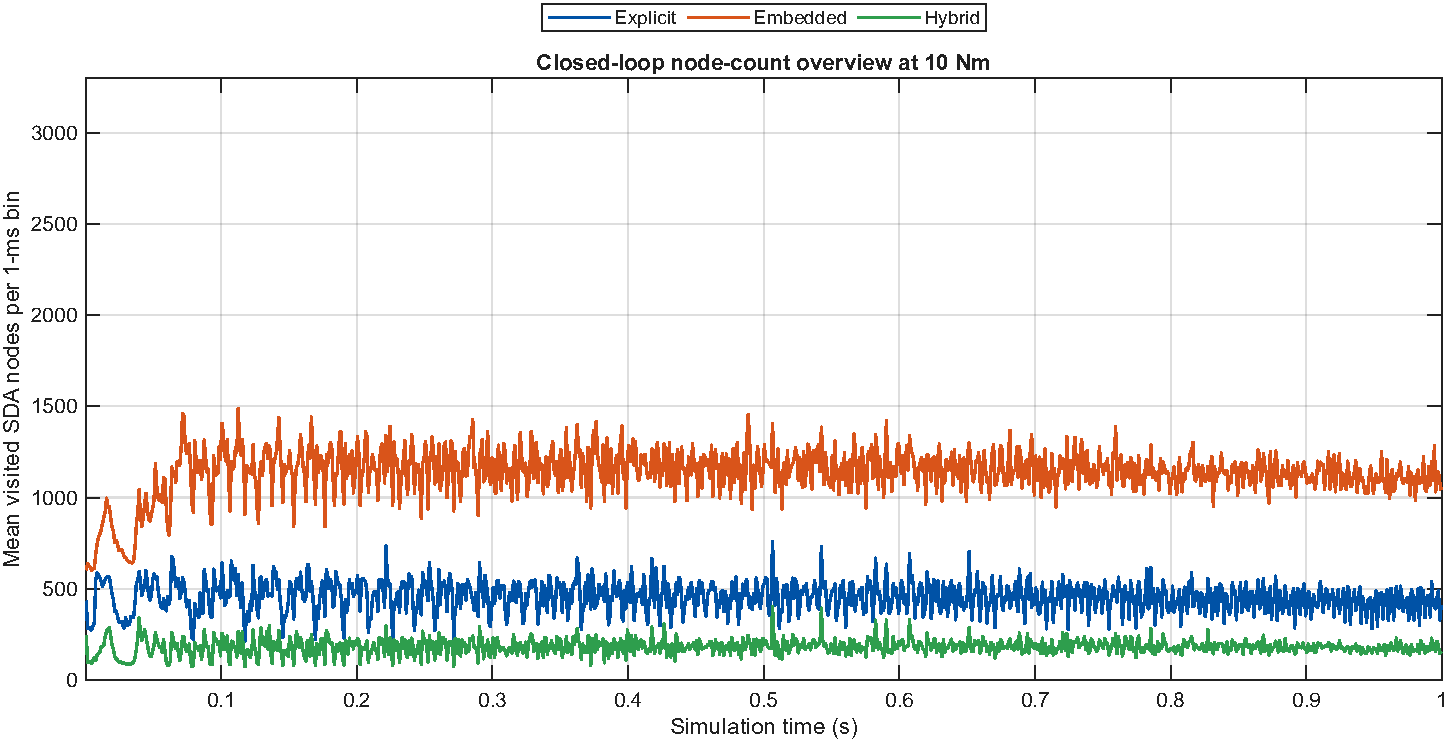
\includegraphics[width=\textwidth]{../hybrid_results/closed_loop_nodes_time_10Nm.pdf}
\caption{Visited-node time series at 10~Nm, displayed as 1-ms bin means over
the complete simulation.}
\label{fig:time_nodes_10}
\end{figure}

\begin{figure}[H]
\centering
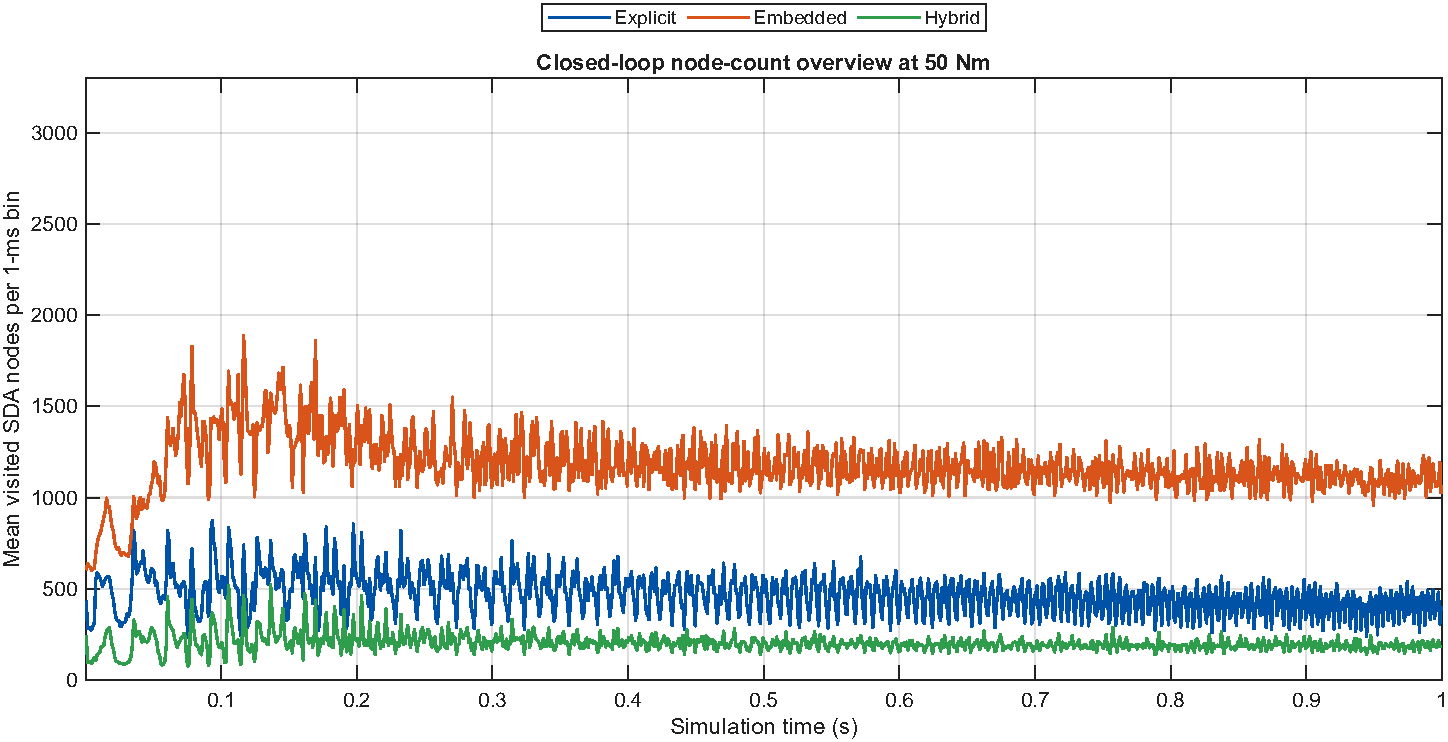
\includegraphics[width=\textwidth]{../hybrid_results/closed_loop_nodes_time_50Nm.pdf}
\caption{Visited-node time series at 50~Nm, displayed as 1-ms bin means over
the complete simulation.}
\label{fig:time_nodes_50}
\end{figure}

\begin{figure}[H]
\centering
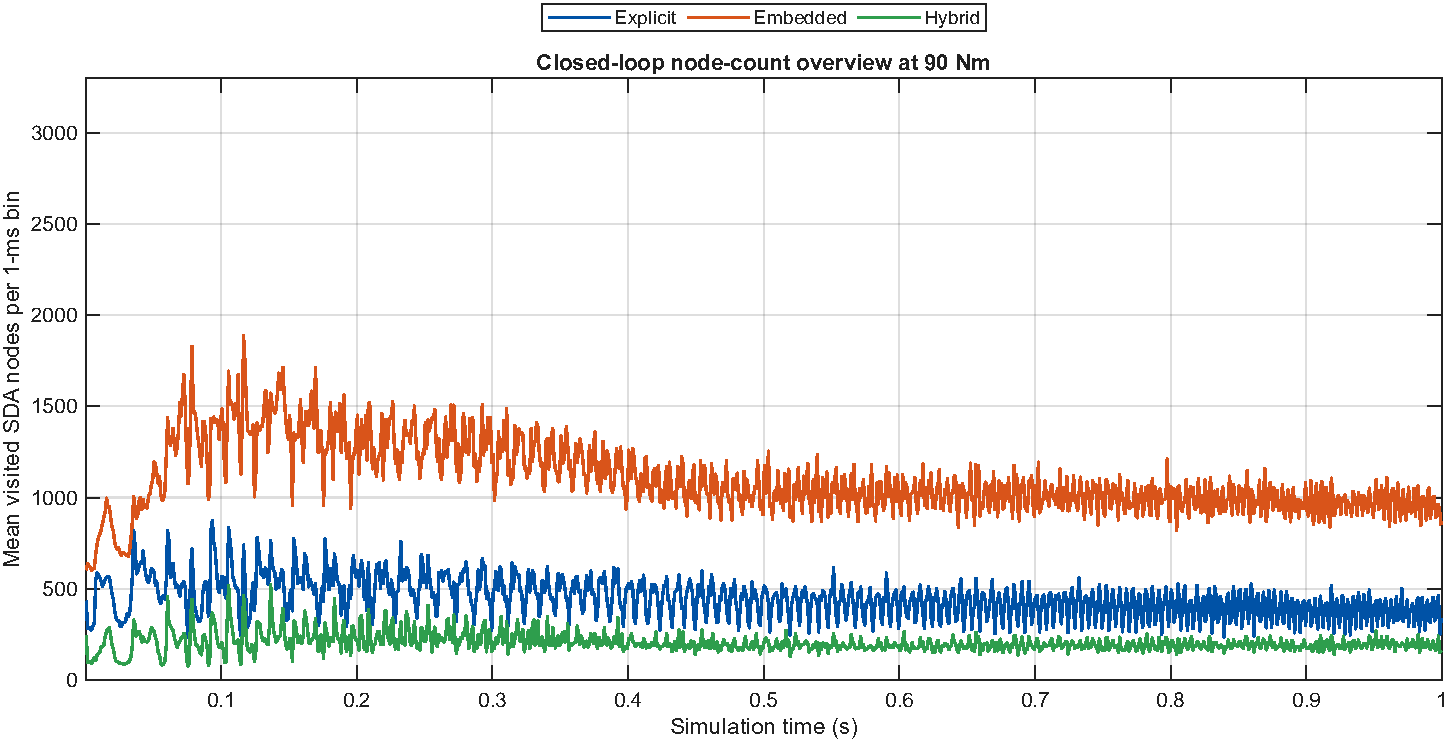
\includegraphics[width=\textwidth]{../hybrid_results/closed_loop_nodes_time_90Nm.pdf}
\caption{Visited-node time series at 90~Nm, displayed as 1-ms bin means over
the complete simulation.}
\label{fig:time_nodes_90}
\end{figure}

Across all three loads, embedded-only search is generally the most expensive,
explicit search is intermediate, and the hybrid is the least expensive.  The
initial transient remains visible in these overview plots but is excluded
from the steady-state statistics below.

\begin{table}[H]
\centering
\caption{Deployed closed-loop search effort over all steady-state
transactions.}
\begin{tabular}{llrrrr}
\toprule
Torque & Method & Mean & Median & Q95 & Maximum\\
\midrule
10~Nm & Explicit & 456.16 & 402 & 930.0 & 2318\\
      & Embedded & 1157.50 & 1162 & 1788.9 & 3110\\
      & Hybrid & \textbf{182.63} & \textbf{138} & \textbf{498.0} & \textbf{1678}\\
50~Nm & Explicit & 469.87 & 416 & 998.0 & 2134\\
      & Embedded & 1197.10 & 1160 & 1872.0 & 3116\\
      & Hybrid & \textbf{204.14} & \textbf{158} & \textbf{500.0} & \textbf{1732}\\
90~Nm & Explicit & 446.87 & 402 & 906.9 & 2030\\
      & Embedded & 1115.40 & 1088 & 1764.0 & 3116\\
      & Hybrid & \textbf{205.57} & \textbf{160} & \textbf{492.0} & \textbf{1696}\\
\bottomrule
\end{tabular}
\end{table}

\begin{figure}[H]
\centering
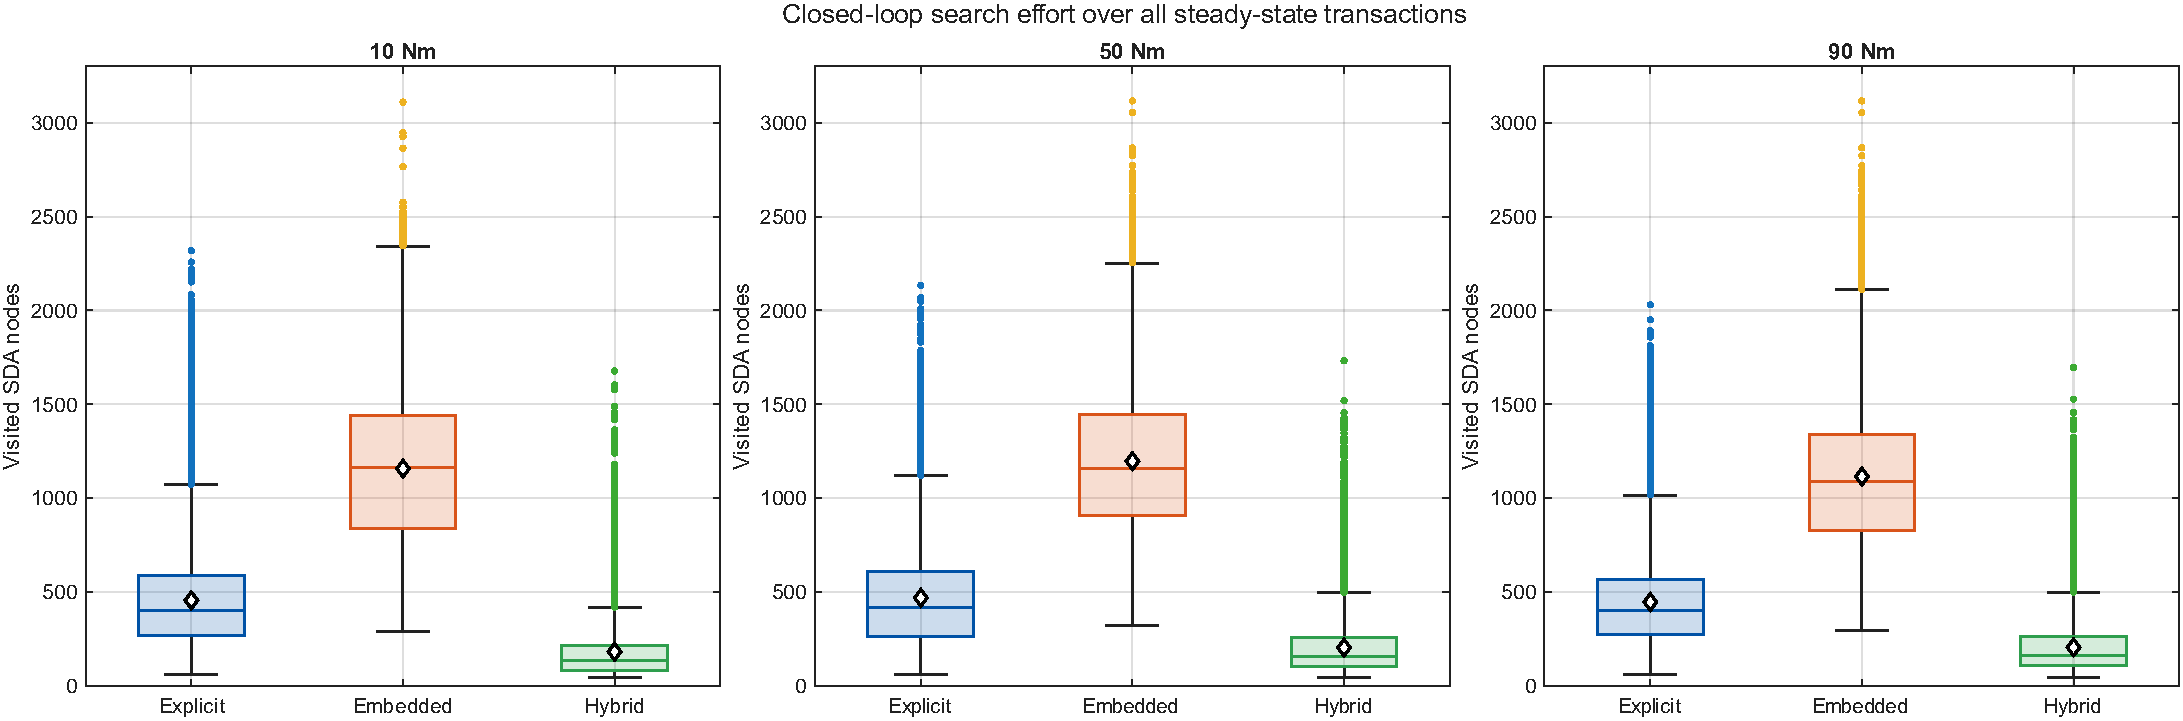
\includegraphics[width=\textwidth]{../hybrid_results/closed_loop_node_distributions.pdf}
\caption{Closed-loop node-count distributions for all retained transactions.}
\end{figure}

The mean reductions relative to native explicit are 59.96\%, 56.55\%, and
54.00\%; relative to embedded-only they are 84.22\%, 82.95\%, and 81.57\%.
The hybrid and both reference formulations select identical optimal sequences
for every paired transaction.  The hybrid--explicit cost difference is below
$1.9\times10^{-12}$, while the median embedded--hybrid difference is exactly
6250 at all three loads.

\begin{table}[H]
\centering
\caption{Embedded-Babai upper-bound quality in closed-loop deployment.}
\resizebox{\textwidth}{!}{%
\begin{tabular}{lrrrr}
\toprule
Torque & Initially optimal & Median $G_0$ & Reduction vs explicit &
Reduction vs embedded\\
\midrule
10~Nm & 52.26\% & $3.4\times10^{-13}$ & 59.96\% & 84.22\%\\
50~Nm & 43.07\% & 36.38 & 56.55\% & 82.95\%\\
90~Nm & 39.37\% & 67.82 & 54.00\% & 81.57\%\\
\bottomrule
\end{tabular}
}
\end{table}

\begin{figure}[H]
\centering
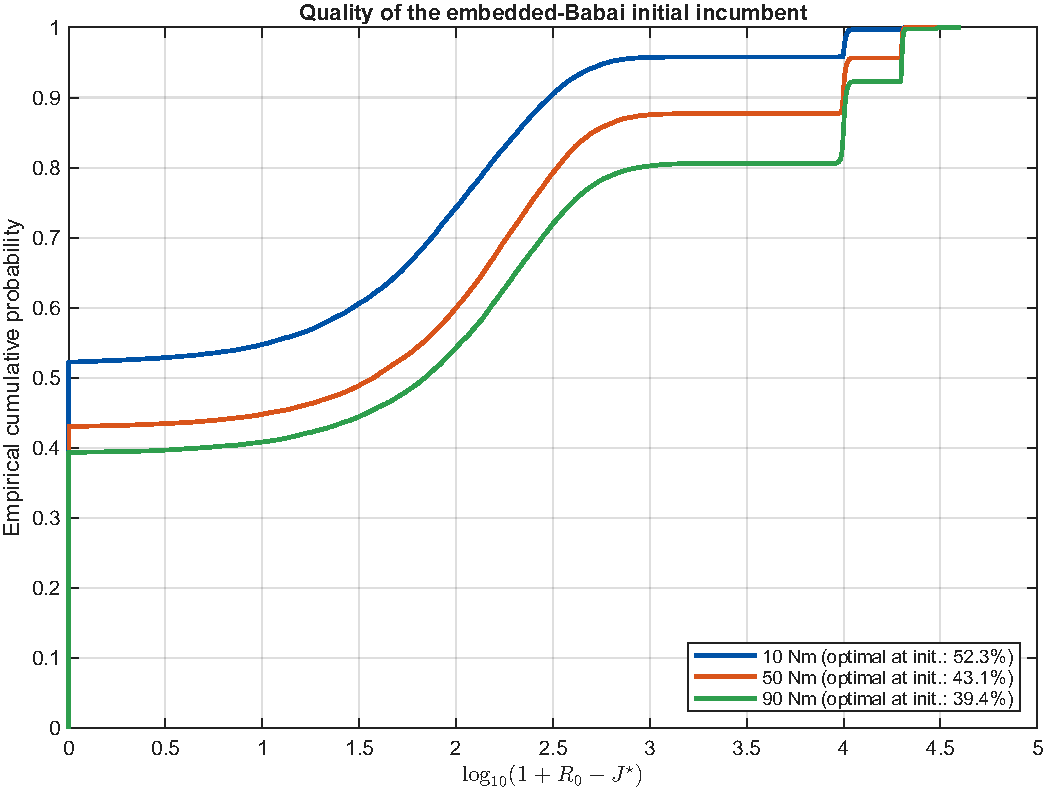
\includegraphics[width=0.88\textwidth]{../hybrid_results/closed_loop_initial_gap_cdf.pdf}
\caption{Empirical distribution of the embedded-Babai initial explicit-cost
gap in the deployed closed-loop controller.}
\end{figure}

A point $(x,y)$ means that the empirical fraction $y$ of transactions obeys
$R_0-J^\star\leq10^x-1$.  This follows from the plotted transformation
\begin{equation}
 X=\log_{10}(1+G_0),\qquad G_0=10^X-1,
\end{equation}
and its empirical cumulative distribution
\begin{equation}
 \widehat F_X(x)=\frac{1}{N}\sum_{k=1}^{N}
 \mathbf{1}\!\left\{\log_{10}(1+G_{0,k})\leq x\right\}.
\end{equation}
Thus, $x=0,1,2,3$ represents $G_0=0,9,99,999$, respectively.  At a fixed
cumulative probability, the curve with the smaller horizontal coordinate
represents the smaller initial gap and hence the tighter initial incumbent.
Equivalently, at a fixed gap threshold, the higher empirical CDF indicates
better initialization quality.  The jump at $x=0$ equals the fraction with zero initial
gap: embedded Babai has already supplied the globally optimal sequence in
those transactions, although the explicit tree must still certify it.

The deployed results therefore reproduce the offline mechanism: embedded Babai
supplies a tight incumbent, while explicit prefix bounds complete the proof
with fewer nodes.  They establish node-count reduction, not yet an equal
processor-time reduction.

\chapter{Conclusion and Scope}

The evidence supports the following chain:
\begin{equation}
\boxed{
\begin{gathered}
\text{complete-sequence equivalence}\\
\Downarrow\\
\text{embedded Babai supplies a tighter feasible upper bound}\\
\Downarrow\\
\text{explicit branch penalties supply more effective certification}\\
\Downarrow\\
\text{the hybrid preserves optimality and reduces visited nodes.}
\end{gathered}}
\end{equation}

The present result establishes search-node reduction, not yet hardware-time
reduction.  Final engineering validation must include the additional embedded
factor construction, Babai pass, memory use, mean execution time, Q99 execution
time, and worst-case execution time relative to the 10/40~kHz deadlines.

Exploratory KDEs, pruning-margin plots, dynamic-radius traces, representative
Q5/Q50/Q95 cases, and full same-prefix distributions remain available in the
detailed analysis report but are not required for the core argument.

\end{document}
